% This must be in the first 5 lines to tell arXiv to use pdfLaTeX, which is strongly recommended.
\pdfoutput=1
\documentclass[11pt]{article}
\usepackage{acl}
\usepackage{times}
\usepackage{latexsym}
\usepackage{soul}
\usepackage{xcolor}
\usepackage{tikz}
\usepackage{pgfplots}
\pgfplotsset{compat=1.17} 
\usepackage[T1]{fontenc}
\usepackage[utf8]{inputenc}
\usepackage{microtype}
\usepackage{amsmath}
\usepackage{algorithm}
\usepackage[noend]{algpseudocode}
\usepackage{CJKutf8}

\title{Multilingual Emotion Recognition in Conversation}

\author{Junyin Chen {} {} {} Hanshu Ding {} {} {} Zoe Fang {} {} {} Yifan Jiang \\
		\texttt{\{junyinc, hsding99, zoekfang, yfjiang\}@uw.edu} \\
        Department of Linguistics \\ University of Washington}

\begin{document}
\maketitle
\begin{abstract}
  We use a multi-task deep learning model to perform emotion recognition in conversation (ERC) task on English and Chinese utterances from TV series scripts. Our experiment shows that adding speaker tags do not improve performance, adding past utterances might add obfuscation, and simple ambiguous utterance is a challenge. Our results show that multilingual training yields better accuracy than monolingual training. We suggest future works to include additional audio data, since the results show that text data limits the interpretability of dialogues.

\end{abstract}

\section{Introduction}
Identification of emotions is one of the core tasks in NLP. As a variant of this task, emotion recognition in conversation, henceforward ERC, is a more difficult task, given that dialogues have a different structure than prose, which is what the majority of the language models are based on. Inspired by past works on ERC, we build a model that predicts emotions on an input utterance. More specifically, we build a multi-task learning model to tackle the complex nature of dialogues, for example multi-party participation and contextual information. We want that the multi-task model can help our model learn dialogue-specific features in hopes that this will improve the accuracy on emotion recognition. To further our project, we adapt our model to predict non-English utterance as well. 

\section{Task Description}

\subsection{Primary Task}
\label{sect:primary_task}

Our primary task is emotion recognition in conversation (ERC) task on the text modality of the Multimodal EmotionLines Dataset (MELD). The dataset is in English and contains dialogues and utterances from TV series scripts . We will predict the emotion for each utterance from dialogues involving multiple speakers.

\subsubsection{Primary Dataset}

MELD \citep{poria-etal-2019-meld} \footnote{\url{https://affective-meld.github.io/}}, also kown as \textit{Multimodel Emotionlines Dataset}, is a multi-party emotional conversational database that is extended from Emotionlines dataset. 
Emotionlines \citep{hsu-etal-2018-emotionlines}\footnote{\url{http://doraemon.iis.sinica.edu.tw/emotionlines/index.html}} dataset is an emotion dialogue dataset with emotion labels for each utterance. The utterances are collected from Friends TV scripts and private Facebook messenger dialogues. Each utterance is labeled with one of Ekman’s six basic emotions plus the neutral emotion. MELD is an upgraded emotion dataset that contains about 13,000 utterances from 1,433 dialogues from only the TV-series Friends. Each utterance in MELD is annotated with emotion and sentiment labels, and encompasses audio, visual, and textual modalities. 
MELD splits the data into training, development, and testing set separately (1039 dialogues for training set, 114 dialogues for developing set and 280 dialogues for testing set). We use the testing set and corresponding gold standard annotation for analysis.

According to Poria, the speakers of these dialogues are categorized to 6 main characters and others. The utterances are distributed relatively evenly with respect to speakers (from 12\% to 16\%).  The emotion distribution for each character is also similar. 

We also use the EmoryNLP \citep{EmoryNLP} as an auxiliary dataset to facilitate the training. EmoryNLP is another multi-party emotional conversational database curated by Zahiri and Choi. The utterances are also collected from the Friends TV show and are annotated with emotion and speaker labels by crowdsourced workers based on Willcox's feeling wheel. EmoryNLP splits the dataset into training, development, and testing sets separately. We use the testing set and corresponding gold standard annotation for analysis. 

According to Zahiri and Choi, the distribution of all emotions in the corpus is not even. The two most dominant emotions, \textit{neutral} and \textit{joyful}, together yield over 50\% of the dataset.

\subsection{Adaptation Task}
\label{sect:adaptation_task}

Our adaptation task is to adapt our model to Chinese dialogues in the Multi-party Dialogue Dataset (MPDD). Other dimensions for this task remain the same as the primary task.

\subsubsection{Dataset}

Multi-party Dialogue Dataset (MPDD) \citep{chen-etal-2020-mpdd} \footnote{\url{http://nlg.csie.ntu.edu.tw/nlpresource/MPDD}} is a Chinese emotional conversational dataset. The dataset contains a total of 25, 548 utterances from 4, 142 dialogues, which are collected from five TV series scripts from \url{www.juban108.com}. Each uttrance is annmotated with three types of labels: emotion, relation, and target listener. In particular, the emotion labels are consistent with those in the Emotionlines dataset.


\section{System Overview}
\label{sec:overview}

\subsection{Design}

Instead of appending the correspondent speaker tag with the utterance for training, we integrate the ideology of having a multi-task deep neural network that shares the lower layer across multiple single-sentence and pairwise text classification tasks. 

With the benefit of multi-task deep neural network, we enable our model to gain context awareness with multiple context related tags, such as speaker, past and future utterance.

\subsection{Methodology}

We want to determine the emotion of a specific utterance in a dialogue group $M$, which contains multiple speakers in speaker group $S$. The dialogue group $M$ can be expressed as a list of vectors: $dialogue = [x_1, x_2, ..., x_{n-1}, x_n]$, where each utterance contains multiple words. The correspondent speaker list can be expressed as another list of vectors: $speaker = [s_1, s_1, ..., s_2, s_3]$, where $s_n$ is in the speaker group $S$. Since this is a supervised setup, we will utilize the manually labeled emotion label $e_n$ corresponding to each utterance $x_n$ in the dialogue group $M$.

The simplest solution is to have a function $f$ that takes each utterance $x_t$ as input and output the correct label $e_t$. For our setup, we decide on a multi-tasking function $f$ to output correspondent speaker $s_t$, as we want to take the speaker into account. Furthermore, we add past utterance $[x_1, x_2, ..., x_{t-1}]$ and even future utterance $[x_{t+1}, x_{t+2}, ..., x_n]$, as we anticipate adding more context around the utterance for analysis will further improve the result.


\subsection{Algorithm}

For each task in the multi-task deep neural network, we use the pretrained "Roberta-base" model \citet{liu-etal-2019-multi}. We choose BERT like algorithms as they both have simple structure, and support more than one segment for tokenization. We choose to use RoBERTa as the main algorithm for training, facilitating result comparison with results listed in \citet{kim-2021-emoberta}. Even though pre-trained BERT and RoBERTa models do not expect more than two segments as inputs, both Kim et al. and us show that having more than two segments improves evaluation results.

We will have either two or three segments, if we want to include both past and future utterances.


\section{Approach}
\label{sec:approach}

\subsection{Problem Statement}
MELD provides information on the speaker and turn ID (in the dialogue) of each utterance. We want to take these two factors into account and build a model that learns emotion prediction based on the context and/or speaker information.


\subsection{Multi-Task Deep Neural Network}

We chose to build a multi-task deep neural network. The shared layer is a RoBERTa base encoder. For the different task heads, we set the main task to be emotion recognition on the MELD data-set, which is also the data-set we run our final evaluation on. The auxiliary task trains parallel to the main task, the point of the auxiliary task is for the model to learn relevant information in addition to the main task. In our model, we have two options for auxiliary task. One of the options is speaker classification, since past literature on emotion recognition in conversation suggest that the models might perform better when they learn speaker-specific features, and we think there might be correlation between each speaker and a certain emotion distribution. The other option for auxiliary task is that we can use data augmentation and run the same emotion classification task, but on additional data-set (EmoryNLP). We can also have more than one auxiliary task, so we run both speaker classification and data augmentation.

\subsection{Input Preprocessing}
Other than the model architecture, our approach also involves specific techniques in input preprocessing. The default input is an utterance in a dialogue, given the turn ID, which is the sequential number in the dialogue, and the speaker information. Since we want to experiment on the impact of speaker information on model performance, we can add a speaker classification auxiliary task, or we can do this in input preprocessing, where we provide the speaker information by concatenating them to the utterance, so that the speaker can potentially be a hint for the model to learn. Another way to preprocess input is to provide context of the utterance. We can provide a certain amount of past or future utterances of the utterance that we want to predict. The caveat of training a MT-DNN on top of RoBERTa is that BERT-like models are previously trained with inputs no longer than two sentences, where each two sentence has a BOS \textit{<s>} token and an EOS \textit{</s>} token. For that reason, when we concatenate more than one past utterance to the to-predict utterance, we strip the EOS token of the past utterances and keep only one that exists between the context and the to-predict utterance. Algorithm~\ref{context} shows our method of adding context and speaker to an utterance.
\begin{algorithm}
\caption{Add All Past Utterance(s)}\label{euclid}
\begin{algorithmic}[1]
\State \textbf{Given} an $Uttr$ and its $idx$ in dialogue
\If {$idx \neq 0$}
    \State $i \gets 1$
    \While {$idx - i \geq 0$}
        \State $Uttr_{past} \gets Data_{idx-i}$
        \State $Speaker_{past} \gets Uttr_{Past_{speaker}}$
        \State $str \gets Speaker_{past} + Uttr_{Past}$
        \State $Context \gets Context + str$
        \State $i \gets i + 1$
    \EndWhile
\EndIf
\State $Uttr \gets Context + EOS + Uttr$
\end{algorithmic}
\label{context}
\end{algorithm}

\subsection{Adaption Task}
As described in the previous section, our adaptation task is performed on MPDD, which is a dialogue corpus in Mandarin. Our approach to this task is similar to the primary task. We build a Multi-Task Deep Neural Network that sets MPDD as the evaluation dataset. We train a multi-task deep neural network for the prediction. As a continuation of the primary task, we only use data augmentation for the auxiliary tasks. We use the same dataset from the primary task for data augmentation, which is MELD and EmoryNLP. The model uses XLM-RoBERTa-lonformer-base as the encoder, since input of MPDD has an average length that is longer than the limit of a roberta-base encoder.
\subsection{Evaluation}

Both tasks will be evaluated using weighted F1 to account for the imbalance of the dataset. We will also evaluate the error rate between predicted the true emotion labels that are labelled manually by the dataset curators. 


\section{Results}
\subsection{Primary results - Monolingual Model}
\label{sec:results}

\begin{table}[hbt]
  \centering
  \begin{tabular}{c|c|c}
    past utterance & future utterance & weighted F1 \\
    \hline
    0 & 0 & 60.17 \\
    \hline
    0 & 6 & 61.96 \\
    \hline
    6 & 0 & \hl{62.46} \\
  \end{tabular}
  \caption{Weighted F1 when number of past or future utterances are added as context. Auxiliary task = Speaker Classification. Speaker in input = True.}
\end{table}

\begin{table}[hbt]
  \centering
  \begin{tabular}{c|c|c}
    speaker task & speaker in input & weighted F1 \\
    \hline
    Yes & No & 63.75 \\
    \hline
    Yes & Yes & 62.92 \\
    \hline
    No & Yes & 62.60 \\
    \hline
    No & No & \hl{64.74} \\
  \end{tabular}
  \caption{Weighted F1 when auxiliary task is speaker classification and/or speaker information is concatenated to input utterance. Number of Past Utterances = 10}
\end{table}

Using our evaluation metric, the model yields a highest 64.74 percent weighted F1 score on MELD. Table 1 shows the results before we add the EmoryNLP dataset, and we have speaker classification task as the auxiliary task. Table 1 shows that adding only past utterances yields the best result. Table 2 shows the results when we set the one of the auxiliary tasks to emotion prediction, while keeping the second auxiliary task of speaker classification optional. We also experiment with the option of having speaker in input.

The prediction output and accuracy of our primary task is shown as below in Table 3 and 4. A major trend we see from the tables is that the prediction for "neutral" has the highest accuracy compared to other emotions. Before data augmentation, the accuracy for the prediction of specific emotion decreases as the quantity of learning instances for the corresponding emotion decreases. After data augmentation, distributional bias in the data-set is not as patent. Specifically, we see a great improvement in "fear" prediction.

\begin{table}[hbt]
  \centering
  \begin{tabular}{c|c|c|c}
    emotion & true count & total count & accuracy \\
    \hline
    neutral & 1026 & 1256 & 0.8169 \\
    \hline
    joy & 247 & 402 & 0.6144 \\
    \hline
    anger & 156 & 345 & 0.4522  \\
    \hline
    surprise & 173 & 281 & 0.6157 \\
    \hline
    sadness & 66 & 208 & 0.3173 \\
    \hline
    disgust & 5 & 68 & 0.0735  \\
    \hline
    fear & 1 & 50 & 0.02 \\
  \end{tabular}
  \caption{MELD Prediction accuracy for each emotion in model with speaker classification task}
\end{table}

\begin{table}[hbt]
  \centering
  \begin{tabular}{c|c|c|c}
    emotion & true count & total count & accuracy \\
    \hline
    neutral & 985 & 1256 & 0.7842 \\
    \hline
    joy & 263 & 402 & 0.6542 \\
    \hline
    anger & 173 & 345 & 0.5014  \\
    \hline
    surprise & 180 & 281 & 0.6429 \\
    \hline
    sadness & 76 & 208 & 0.3654\\
    \hline
    disgust  & 13 & 68 & 0.1912  \\
    \hline
    fear & 11 & 50 & 0.22 \\
  \end{tabular}
  \caption{MELD Prediction accuracy for each emotion in best-performing model}
\end{table}

\begin{figure*}
\centering
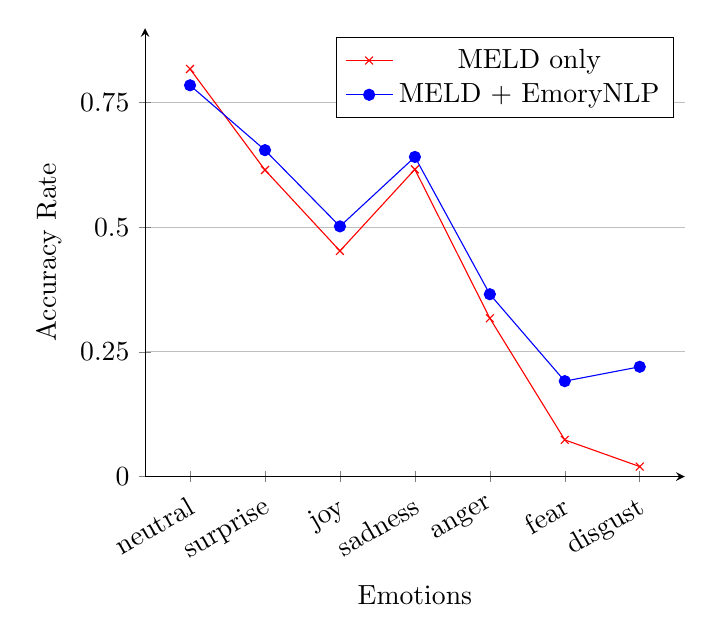
\begin{tikzpicture}
      \begin{axis}[
        axis x line=bottom,
        axis y line=left,
        ymajorgrids=true,
        %
        ylabel=Accuracy Rate,
        ymin=0,
        ytick={0,0.25,0.50,0.75,1.00},
        enlargelimits=auto,
        %
        xlabel= Emotions,
        xtick={1,2,...,7},
        xticklabels={{neutral},{surprise}, {joy}, {sadness},{anger},{fear},{disgust}},
        x tick label style={rotate=30,anchor=north east},
        ]
        \addplot[color=red,mark=x]
          plot coordinates {
            (1,0.8169)
            (2,0.6144)
            (3,0.4522)
            (4,0.6157)
            (5,0.3173)
            (6,0.0735)
            (7,0.02)
          };
          \addlegendentry{MELD only}
                
      \addplot[color=blue,mark=*]
          plot coordinates {
            (1,0.7842)
            (2,0.6542)
            (3,0.5014)
            (4,0.6406)
            (5,0.3654)
            (6,0.1912)
            (7,0.22)
          };
          \addlegendentry{MELD $+$ EmoryNLP}
      \end{axis}
    \end{tikzpicture}
\caption{Accuracy Comparison before and after Data Augmentation}

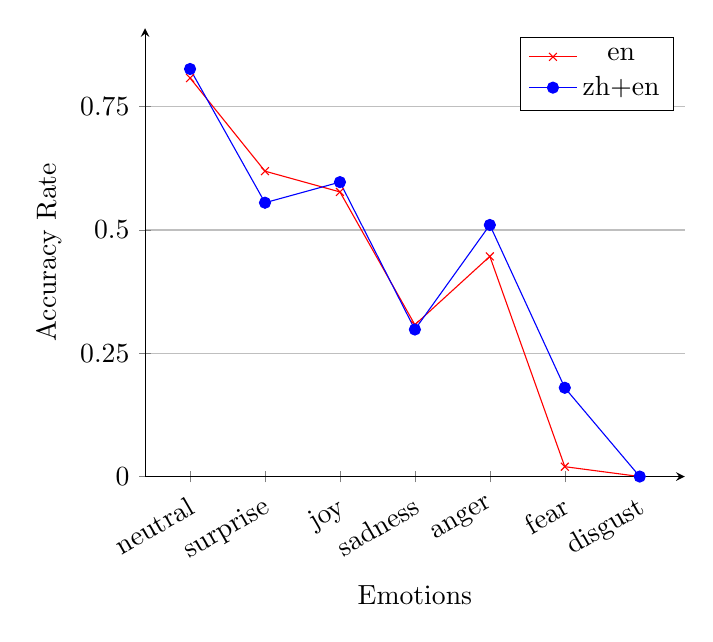
\begin{tikzpicture}
      \begin{axis}[
        axis x line=bottom,
        axis y line=left,
        ymajorgrids=true,
        %
        ylabel=Accuracy Rate,
        ymin=0,
        ytick={0,0.25,0.50,0.75,1.00},
        enlargelimits=auto,
        %
        xlabel= Emotions,
        xtick={1,2,...,7},
        xticklabels={{neutral},{surprise}, {joy}, {sadness},{anger},{fear},{disgust}},
        x tick label style={rotate=30,anchor=north east},
        ]
        \addplot[color=red,mark=x]
          plot coordinates {
            (1,0.8081)
            (2,0.6192)
            (3,0.5771)
            (4,0.3077)
            (5,0.4464)
            (6,0.02)
            (7,0)
          };
          \addlegendentry{en}
                
      \addplot[color=blue,mark=*]
          plot coordinates {
            (1,0.8264)
            (2,0.5552)
            (3,0.597)
            (4,0.2981)
            (5,0.5101)
            (6,0.18)
            (7,0)
          };
          \addlegendentry{zh$+$en }
      \end{axis}
    \end{tikzpicture}
\caption{Accuracy Comparison Between English Only Training Set and Multi-lingual Training Set (eval on MELD)}

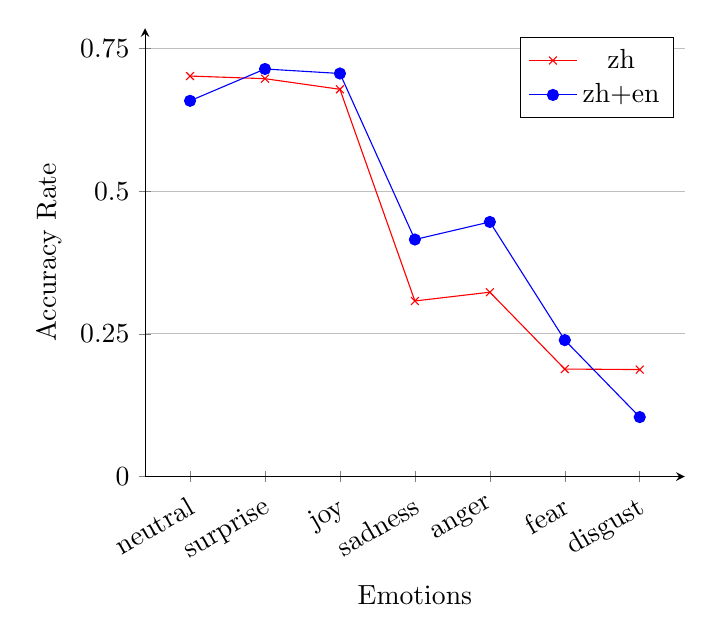
\begin{tikzpicture}
      \begin{axis}[
        axis x line=bottom,
        axis y line=left,
        ymajorgrids=true,
        %
        ylabel=Accuracy Rate,
        ymin=0,
        ytick={0,0.25,0.50,0.75,1.00},
        enlargelimits=auto,
        %
        xlabel= Emotions,
        xtick={1,2,...,7},
        xticklabels={{neutral},{surprise}, {joy}, {sadness},{anger},{fear},{disgust}},
        x tick label style={rotate=30,anchor=north east},
        ]
        \addplot[color=red,mark=x]
          plot coordinates {
            (1,0.7019)
            (2,0.6973)
            (3,0.6787)
            (4,0.3077)
            (5,0.3231)
            (6,0.1884)
            (7,0.1875)
          };
          \addlegendentry{zh}
                
      \addplot[color=blue,mark=*]
          plot coordinates {
            (1,0.6585)
            (2,0.7143)
            (3,0.7064)
            (4,0.4154)
            (5,0.4462)
            (6,0.2391)
            (7,0.1042)
          };
          \addlegendentry{zh$+$en}
      \end{axis}
    \end{tikzpicture}
\caption{Accuracy Comparison Between English Only Training Set and Multi-lingual Training Set (eval on MPDD)}
\end{figure*}

\subsection{Adaptation Task - Multilingual Model}

\begin{table}[hbt]
  \centering
  \begin{tabular}{c|c|c}
    evaluation & training & weighted F1 \\
    \hline
    MELD & zh$+$en & 62.88 \\
    \hline
    MELD & en & 61.18 \\
    \hline
    MPDD & zh$+$en & 59.73 \\
    \hline
    MPDD & zh & 57.93
  \end{tabular}
  \caption{Weighted F1 for Adaption Task. Shared encoder=xlm-roberta}
\end{table}


Table 5 shows the weighted F1 of both monolingual and multilingual models. The results show that multilingual training datasets yield better results than monolingual training datasets.

\section{Discussion}

\subsection{Pre-trained model decision}

We choose to use the xlm-roberta-longformer-base model, instead of the RoBERTa model used by Kim et al, due to the utterance length in the MPDD dataset. One utterance in MPDD dataset usually contains several long sentences, whereas the utterance in MELD or EmoryNLP usually contains only one sentence. If we choose to segment sentences in the MPDD utterances, we need to perform sentiment analysis on those newly segmented sentences, which is time-consuming. Instead, we use the xlm-roberta-longformer-base model since it is trained in multiple languages, including Chinese, and can process longer sentences as input.

\subsection{Qualitative Analysis}

\subsubsection{MELD}

We did a qualitative analysis with ten correctly and ten incorrectly classified random samples from the evaluation dataset of MELD.

{\small
\begin{quote}

<s>Joey:You know, I think I was sixteen. \hl{Monica}:Please, just \hl{a} little bit off the back. \hl{Ph}oe\hl{be}:I\'m still on "no." \hl{</s></s>Uh,} \hl{morning}. \hl{Do} \hl{you} guys think \hl{you} \hl{could} \hl{close} \hl{your} eyes \hl{for} \hl{just} a \hl{sec}\hl{?</s>}

\end{quote}

A correctly classified example when training with speaker context. Both the prediction and truth are 'neutral'. The predicted speaker is Monica, and the true speaker is Rachel.

\begin{quote}

\hl{<s>}\hl{Rachel}:It's not a purse! It's a shoulder bag\hl{.} \hl{Joey}:It looks like a women's purse\hl{.} \hl{Rachel}:\hl{No} \hl{Joey}, look. Trust me, all the men are wearing them in the spring catalog\hl{.} Look\hl{.} See look, \hl{Joey}:See look, \hl{</s></s>Exactly!} \hl{Unisex!</s>}

\end{quote}

An incorrectly classified example when training with speaker context. The prediction is 'joy' while the truth is 'neutral'. The predicted and the true speaker is Rachel.}

We initially anticipate that the speaker tag will be utilized for sentiment classification. However, after using EmoryNLP for auxiliary emotion and speaker detection tasks, we notice an increase in accuracy in the emotion detection task. However, the speaker contexts are mainly utilized by incorrect outputs. Our manual inspections show that only 5 of the correct samples focus on the speaker tags in the last layer, whereas all incorrect samples focus on the speaker tags in the last layer. Both correct and incorrect samples have sixty percent accuracy in predicting the speaker. This phenomenon far deviates from Kim et al.'s result, that <s> token mainly focus on the speaker in correctly classified examples. Based on the new finding, we revised our hypothesis, that adding speaker contexts does not improve the emotion detection accuracy. We then train a new model without the speaker context.

{\small
\begin{quote}

<s>Joey:You know, I think I was sixteen. \hl{Monica}:Please, just \hl{a} little bit off the back. \hl{Ph}oe\hl{be}:I\'m still on "no." \hl{</s></s>Uh,} \hl{morning}. \hl{Do} \hl{you} guys think \hl{you} \hl{could} \hl{close} \hl{your} eyes \hl{for} \hl{just} a \hl{sec}\hl{?</s>}

\end{quote}

A correctly classified example when training without speaker context. Both the prediction and truth are 'joy'.

\begin{quote}

\hl{<s>} And you’re upset because \hl{you} didn’t \hl{make} your best friend \hl{cry}? I mean, all \hl{I}’m asking for is just a \hl{little emotion! Is that too} much to \hl{ask} after six years\hl{?!}\hl{</s></s>} \hl{I mean what}\hl{?</s>}

\end{quote}

An incorrectly classified example when training without speaker context. The prediction is 'joy' while the truth is 'sadness'.}

Our manual inspections of the new model suggest speaker context is unnecessary when adding a dataset. Nine correct samples and five incorrect samples focus on the previous utterances in the last layer. The incorrect samples usually contain words that are usually associated with the predicted semantic labeling, but when combined with important sentiment keywords, the result becomes opposite. For example, as the incorrect sample listed above, \textit{cry}, \textit{emotion}, and \textit{too} are used in the previous utterances, which can be associated with joy, but with \textit{upset}, the true sentiment becomes sadness.

\subsubsection{MPDD}
We also did a qualitative analysis with ten correctly and ten incorrectly classified random samples from the evaluation dataset split of the MPDD dataset.


\begin{CJK*}{UTF8}{bsmi}
{\small
\begin{quote}

<s> 應該願意作,比你還願意作。 那可不一定,聽說要抽血,可能就不願意了。 你跟\underline{韓東}說了嗎? 說了。 光說\underline{不行},你得催着點,要不得拖到啥時候? 別光說\underline{我}\underline{的事},\underline{你也}該給你的\underline{親爸}盡盡\underline{孝心}\underline{了吧}? \underline{</s></s> 我的親爸?</s>}
\end{quote}

A correctly classified example when training without speaker context. Both the prediction and truth are 'joy'.

\begin{quote}

<s> \underline{八萬}是\underline{多少}? 八萬就是八萬。 八萬\underline{就}八萬吧。\underline{咱}們\underline{就}去\underline{取}吧,在哪兒取? 在\underline{鎮}政府。 那\underline{好吧},咱們\underline{這}就去。 要帶上\underline{您}的身份證和戶口本\underline{。 </s></s> 行。</s>}

\end{quote}

An incorrectly classified example when training without speaker context. The prediction is 'joy' while the truth is 'neutral'.}
\end{CJK*} 

\begin{CJK*}{UTF8}{bsmi}
Seven of the correct sample, and three of the incorrect sample focus on the past utterance in the last layer. Noticeably, the model struggles with short, simple, but sometimes ambiguous utterances. For example, as the incorrect sample listed above, the utterance for judgement is just one Chinese character, \textit{行}, which means Okay in English. \textit{行} does carry multiple meanings, but means acknowledging the previous utterance in this case, which the model incorrectly predicted the sentence as joy, while the truth in neutral.
\end{CJK*} 



\section{Conclusion}
\label{sect:conclusion}

In this paper, we showed how to utilize multi-task deep learning model to perform emotion recognition in conversation (ERC) task. Our also showed that multilingual training datasets yield better results than monolingual training dataset. Our manual inspections on model's last layer suggest adding additional textual contexts, such as speaker tags, does not improve the performance. We suggest future works to include additional non-textual contexts, such as audio or video data, since the results show that text data limits the interpretability of dialogues.

% Entries for the entire Anthology, followed by custom entries
\bibliography{anthology, custom}

\end{document}